\achapter{1}{Introduction to Systems of Linear Equations}\label{sec:intro_linear_systems}


\vspace*{-17 pt}
\framebox{
\parbox{\dimexpr\linewidth-3\fboxsep-3\fboxrule}
{\begin{fqs}
\item What is a linear equation?
\item What is a system of linear equations?
\item What is a solution set of a system of linear equations?
\item What are equivalent systems of linear equations?
\item What operations can we use to solve a system of linear equations?
\end{fqs}}}%\hspace*{3 pt}}

\vspace*{13 pt}

\csection{Application: Electrical Circuits}

Linear algebra is concerned with the study of systems of linear equations. There are two important aspects to linear systems. One is to use given information to set up a system of equations that represents the information (this is called \emph{modeling}), and the other is to solve the system.  As an example of modeling, we consider the application to the very simple electrical circuit. An electrical circuit consists of
\begin{itemize}
\item one or more electrical sources, denoted by \ \ \  \resizebox{!}{0.25in}{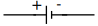
\includegraphics{1_a_pa_source}}
\item one or more resistors, denoted by \ \ \ 
\resizebox{!}{0.25in}{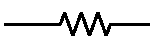
\includegraphics{1_a_pa_resistor}}.
\end{itemize}
A source\index{circuits!source} is a power supply like a battery, and a resistor\index{circuits!resistor} is an object that consumes the electricity, like a lamp or a computer. A simple circuit consists of one or more sources connected to resistors, like the one shown in Figure \ref{F:circuit1}. The straight lines in the circuit indicate wires through which current flows. The points labeled P and Q are called \emph{junctions} or \emph{nodes}\index{circuits!junctions}.
\begin{figure}[h]
\begin{center}
\resizebox{!}{2.5in}{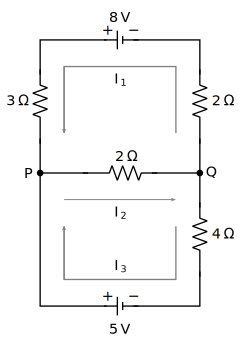
\includegraphics{1_a_pa_circuit1.eps}}
\end{center}
\caption{A circuit.}
\label{F:circuit1}
\end{figure}

The source creates a charge that produces potential energy $E$ measured in volts (V).  Current flows out of the positive terminal of a source and runs through each branch of the circuit. Let $I_1$, $I_2$, and $I_3$ be the currents as illustrated in  Figure \ref{F:circuit1}. The goal is to find the current flowing in each branch of the circuit.  

Linear algebra comes into play when analyzing a circuit based on the relationship between current $I$, resistance $R$, and voltage $E$. There are laws governing electrical circuits that state that $E = IR$ across a resistor. Additionally, Kirchoff's Current and Voltage Laws indicate how current behaves within the whole circuit. Using all these laws together, we derive the system
\begin{alignat}{4}
{}I_1 \	&- \	&{}I_2 \	&+ \	&{}I_3 \	&= 0  \notag \\ %\label{eq:circuit_1} \\
5I_1 \	&+ \	&2I_2 \		&{} \ 	&{}  \		&= 8 \notag \\ %\label{eq:circuit_2} \\
	\	&{} \ 	&2I_2 \		&+ \	&4I_3 \		&= 5, \notag %\label{eq:circuit_3}
\end{alignat}
where $I_1$, $I_2$, and $I_3$ are the currents at the points indicated in Figure \ref{F:circuit1}. To finish analyzing the circuit, we now need to solve this system. In this section we will begin to learn systematic methods for solving systems of linear equations. More details about the derivation of these circuit equations can be found at the end of this section.  

\csection{Introduction}

Systems of linear equations  arise in almost every field of study: mathematics, statistics, physics, chemistry, biology, economics, sociology, computer science, engineering, and many, many others. We will study the theory behind solving systems of linear equations, implications of this theory, and applications of linear algebra as we proceed throughout this text. 

\begin{pa} \label{pa:1_a} ~
\be
\item \label{ex:system_1} Consider the following system of two linear equations in two unknowns, $x_1, x_2$: 
\begin{alignat}{4}
2x_1	&{}-{}	&3x_2 	&= 0  \notag \\%\label{eq:PA1.1_1} \\
x_1 	&{}-{} 	&x_2		&= 1. \notag %\label{eq:PA1.1__2} 
\end{alignat}


One way to solve such a system of linear equations is the method of substitution (where one equation is solved for one variable and then the resulting expression is substituted into the remaining equations). This method works well for simple systems of two equations in two unknowns, but becomes complicated if the number or complexity of the equations is increased. 

Another method is elimination -- the method that we will adopt in this book. Recall that the elimination method works by multiplying each equation by a suitable constant so that the coefficients of one of the variables in each equation is the same. Then we subtract corresponding sides of these equations to eliminate that variable. 

Use the method of elimination to show that this system has the unique solution $x_1=3$ and $x_2=2$. Explain the specific steps you perform when using elimination. 

\item Recall that a linear equation in two variables can be represented as a line in $\R^2$, the Cartesian plane, where one variable corresponds to the horizontal axis and the other to the vertical axis. Represent the two equations $2x_1 -3x_2 = 0$ and $x_1 - x_2= 1$ in $\R^2$ and illustrate the solution to the system in your picture.

\item The previous example should be familiar to you as a system of two equations in two unknowns. Now we consider a system of three equations in three unknowns 
\begin{alignat}{4}
{}I_1 	&{}-{} 	&{}I_2	&{}+{}	&{}I_3 	&{}={} 	&0&{}  \label{eq:PAcircuit_a} \\
{5}I_1 	&{}+{}	&{2}I_2 	&{} 		&{} 		&{}={}	&8&{} \label{eq:PAcircuit_b} \\
{}		&{} 	 	&{2}I_2 	&{}+{}	& {4}I_3	&{}={}	&5&{} \label{eq:PAcircuit_c}
\end{alignat}
that arises from our electrical circuit in Figure \ref{F:circuit1}, with currents $I_1$, $I_2$, and $I_3$ as indicated in the circuit. 
\begin{figure}[h]
\begin{center}
\resizebox{!}{2.5in}{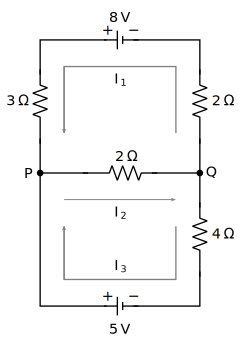
\includegraphics{1_a_pa_circuit1.eps}}
\end{center}
\caption{A circuit.}
\label{F:circuit1}
\end{figure}
In the remainder of this preview activity we will apply the method of elimination to solve the system of linear equations (\ref{eq:PAcircuit_a}), (\ref{eq:PAcircuit_b}), and (\ref{eq:PAcircuit_c}). 

    \ba
            \item Replace equation (\ref{eq:PAcircuit_b}) with the new equation obtained by multiplying both sides of equation (\ref{eq:PAcircuit_a}) by 5 and then subtracting corresponding sides of this equation from the appropriate sides of equation (\ref{eq:PAcircuit_b}).  Show that the resulting system is
        \begin{alignat}{4}
{}I_1 \	&- \	&{}I_2 \	&+ \	&{}I_3 \	&= 0  \notag \\
     \	&  \	&7I_2  \		&{-} \ 	&{5}I_3  \		&= 8 \label{eq:PAcircuit_d} \\
	\	&{} \ 	&2I_2 \		&+ \	&4I_3 \		&= 5. \notag
    \end{alignat}


         \item Now eliminate the variable $I_2$ from the last two equations in the system in part (a) by using equations (\ref{eq:PAcircuit_c}) and (\ref{eq:PAcircuit_d}) to show that $I_3=0.5$. Explain your process. 

        \item Once you know the value for $I_3$, how can you find $I_2$? Then how do you find $I_1$? Use your method to show that the solution to this system is the ordered triple (1,1.5,0.5). Interpret the result in terms of currents. 

	\ea

\ee

\end{pa}

\csection{Notation and Terminology}

To study linear algebra, we will need to agree on some general notation and terminology to represent our systems. 

An equation like $4x_1 + x_2 = 8$ is called a linear equation because the variables ($x_1$ and $x_2$ in this case) are raised to the first power, and there are no products of variables. The equation $4x_1 + x_2 = 8$ is a linear equation in two variables, but we can make a linear equation with any number of variables we like. 

\begin{definition} A \textbf{linear equation}\index{linear equation} in the variables $x_1$, $x_2$, $\ldots$, $x_n$ is an equation of the form
\[a_1x_1 + a_2x_2 + \cdots + a_nx_n = b,\]
where $n$ is a positive integer and $a_1$, $a_2$, $\ldots$, $a_n$ and $b$ are constants. The constants $a_1$, $a_2$, $\ldots$, $a_n$ are called the \textbf{coefficients}\index{linear equation!coefficients} of the equation. 
\end{definition}

We can use any labels for the variables in a linear equation that we like, e.g., $I_1$, $x_1$, $t_1$, and you should become comfortable working with variables in any form. We will usually use subscripts, as in $x_1, x_2, x_3, \ldots$, to represent the variables as this notation allows us to have any number of variables. Other examples of linear equations are 
\[ x+2y=4 \quad \text{ and } \quad \sqrt{2}x_1-3x_2=\frac{1}{4}x_3+\pi \, .\]
On the other hand, the equations
\[\frac{1}{x}+y-z=0 \quad \text{ and } \quad 2x_1=\sqrt{x_2}-5 \]
are non-linear equations. 

\begin{definition} A \textbf{system of linear equations}\index{system of linear equations} is a collection of one or more linear equations in the same variables. 
\end{definition}

For example, the two equations 

\begin{equation} \label{eq:1_a_PA_1}
\begin{alignedat}{4}
x_1 	&{}-{}	&x_2	&= 1  \\ 
2x_1 	&{}+{} 	&x_2	&= 5 
\end{alignedat}
\end{equation}
form a system of two linear equations in variables $x_1$, $x_2$.

\begin{definition} A \textbf{solution}\index{system of linear equations!solution} to a system of linear equations is an ordered $n$-tuple $(s_1, s_2, \ldots, s_n)$ of numbers so that we obtain all true statements in the system when we replace the variable in order with $s_1$, $s_2$, $\ldots$, and  $s_n$. 
\end{definition}

For example, $x_1=2, x_2=1$, or simply $(2,1)$, is a solution to the above system of linear equations in \eqref{eq:1_a_PA_1} as can be checked by substituting the variables into each equation. In solving a system of linear equations, we are interested in finding the set of all solutions, which we will call the \emph{solution set of the system}\index{system of linear equations!solution set}. For the above system in \eqref{eq:1_a_PA_1}, the solution set is the set containing the single point $(2,1)$, denoted $\{(2,1)\}$, because there is only one solution. If we consider just the equation $x_1-x_2=0$ as our system, the solution set is the line $x_1=x_2$ in the plane. More generally, a set of solutions is a collection of ordered $n$-tuples of numbers. We denote the set of all ordered $n$-tuples of numbers as $\R^n$. So, for example, $\R^2$ is the set of all ordered pairs, or just the standard coordinate plane, and $\R^3$ is the set of all ordered triples, or the three-dimensional space. 


\csection{Solving Systems of Linear Equations}

In Preview Activity \ref{pa:1_a}, we were introduced to linear systems and the method of elimination for a system of two or three variables. Our goal now is to come up with a systematic method that will reduce any linear system to one that is easy to solve without changing the solution set of the system. Two linear systems will be called \emph{equivalent}\index{system of linear equations!equivalent systems} if they have the same solution set. 

The operations we used in Preview Activity \ref{pa:1_a} to systematically eliminate variables so that we can solve a linear system are called \emph{elementary operations on a system of linear equations} or just \emph{elementary operations}\index{elementary operations}\index{system of linear equations!operations}. In the exercises you will argue that elementary operations do not change the solution set to a system of linear equations, a fact that is summarized in the following theorem.

\begin{theorem} The \textbf{elementary operations} on a system of linear equations: 
\begin{enumerate}
\item replacing one equation by the sum of that equation and a scalar multiple of another equation;
\item interchanging two equations;
\item replacing an equation by a nonzero scalar multiple of itself;
\end{enumerate}
do not change the solution set to the system of equations.
\end{theorem}

When we apply these elementary operations our ultimate goal is to produce a system of linear equations in a simplified form with the same solution set, where the number of variables eliminated from the equations increase as we move from top to bottom. This method is called the \emph{elimination}\index{system of linear equations!elimination} method. 

\begin{activity} For systems of linear equations with a small number of variables, many different methods could be used to find a solution. However, when a system gets large, ad-hoc methods become unwieldy. One of our goals is to develop an algorithmic approach to solving systems of linear equations that can be programmed and applied to any linear system, so we want to work in a very prescribed method as indicated in this activity. Ultimately, once we understand how the algorithm works, we will use calculators/computers to do the work. Apply the elimination method as described to show that the solution set of the following system is $(2, -1, 1)$:
\begin{alignat*}{4}
x_1 &{}+{}& x_2 &{}-{}& x_3 &= 0   \\
2x_1 &{}+{}& x_2 &{}-{}& x_3 &= 2  \\
x_1&{}-{}&x_2 &{}+{}& 2x_3 &= 5. 
\end{alignat*}
	\ba
	\item Use the first equation to eliminate the variable $x_1$ in the second and third equations.
	
	\item Use the new second equation to eliminate the variable $x_2$ in the third equation and find the value of $x_3$. 
	
	\item Find values of $x_2$ and then $x_1$.

	
	\ea
	
\end{activity}



\noindent \textbf{Important Note:} Technically, we don't really add two equations or multiply an equation by a scalar. When we refer to a scalar multiple of an equation, we mean the equation obtained by equating the scalar multiple of the expression on the left side of the equation and the same scalar multiple of the expression on the right side of the equation. Similarly, when we refer to a sum of two equations, we don't really add the equations themselves. Instead, we mean the equation obtained by equating the sum of the expressions on the left sides of the equations to the sum of the expressions on the right sides of the equations. We will use the terminology ``scalar multiple of an equation" and ``sum of two equations" as shorthand to mean what is described here.


\noindent \textbf{Another Important Note:} There is an important and subtle point to consider here. When we use these operations to find a solution to a system of equations, we are assuming that the system has a solution. The application of these operations then tells us what a solution must look like. However, there is no guarantee that the outcome is actually a solution -- to be safe we should check to make sure that our result is a solution to the system. In the case of linear systems, though, every one of our operations on equations is reversible (if applied correctly), so the result will always be a solution (but this is not true in general for non-linear systems).  


\noindent \textbf{Terminology:} A system of equations is called \emph{consistent}\index{system of linear equations!consistent} if the system has at least one solution. If a system has no solutions, then it is said to be \emph{inconsistent}\index{system of linear equations!inconsistent}.

\csection{The Geometry of Solution Sets of Linear Systems}

We are familiar with linear equations in two variables from basic algebra and calculus (through linear approximations). The set of solutions to a system of linear equations in two variables has some geometry connected to it.


\begin{activity} \label{act:1_a_2} Recall that we examined the geometry of the system 
\begin{alignat}{4}
2x_1 	&{}-{}	&3x_2 	&= 0  \notag \\%\label{eq:PA1.1_1} \\
x_1 	&{}-{} 	&x_2		&= 1 \notag %\label{eq:PA1.1__2} 
\end{alignat}
in Preview Activity \ref{pa:1_a} to show that the resulting solution set consists of a single point in the plane.

In this activity we examine the geometry of the system 
\begin{equation}\label{eq:1_a_2}
\begin{alignedat}{4}
{2}x_1 	&{}-{}	&{}x_2 	&= 1&{}  \\ %\notag \\%\label{eq:PA1.1_1} \\
{2}x_1 	&{}-{} 	&{2}x_2		&= 2&{.} % \notag %\label{eq:PA1.1__2} 
\end{alignedat}
\end{equation}
\ba
\item Consider the linear equation $2x_1-2x_2=2$ (or, equivalently $2x-2y=2$). What is the graph of the solution set (the set of points $(x_1, x_2)$ satisfying this equation) of this single equation in the plane? Draw the graph to illustrate. 


\item How can we represent the solution set of the system \eqref{eq:1_a_2} of two equations graphically? How is this solution set related to the solution set of the single equation $2x_1-2x_2=2$? Why? How many solutions does the system \eqref{eq:1_a_2} have? 


\item There are exactly three possibilities for the number of solutions to a general system of two linear equations in two unknowns. Describe the geometric representations of solution sets for each of the possibilities. Illustrate each with a specific example (of your own) using a system of equations and sketching its geometric representation. 

\ea

\end{activity}

Activity \ref{act:1_a_2} shows that there are three options for the solution set of a system: A system can have no solutions, one solution, or infinitely many solutions.


Now we consider systems of three variables. As an example, let us look at the linear equation $x+y+z=1$ in the three variables $x$, $y$, and $z$. Notice that the points $(1,1,-2)$, $(0,0,0)$, and $(-1,-1,2)$ all satisfy this equation. As a linear equation, the graph of $x+y+z=0$ will be a plane in three dimensions that contains these three points, as shown in Figure \ref{F:1_a_plane}. Hence when we consider a linear system in three unknowns, we are looking for a point in the three dimensional space that lies on all the planes described by the equations. 

\begin{figure}[h]
\begin{center}
\resizebox{!}{2.0in}{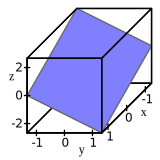
\includegraphics{1_a_plane.eps}}
\caption{The plane $x+y+z=1$.}
\label{F:1_a_plane}
\end{center}
\end{figure}

\begin{activity} \label{act:1_a_3} In this activity we examine the geometry of linear systems of three equations in three unknowns. Recall that each linear equation in three variables has a plane as its solution set. Use a piece of paper to represent each plane. 
\ba
\item Is it possible for a general system of three linear equations in three unknowns to have no solutions? If so, geometrically describe this situation and then illustrate each with a specific example using a system of equations. If not, explain why not.


\item Is it possible for a general system of three linear equations in three unknowns to have exactly one solution? If so, geometrically describe this situation and then illustrate each with a specific example using a system of equations. If not, explain why not.
 

\item Is it possible for a general system of three linear equations in three unknowns to have infinitely many solutions? If so, geometrically describe this situation and then illustrate each with a specific example using a system of equations. If not, explain why not.

 


\ea

\end{activity}


\csection{Examples}

\ExampleIntro

\begin{example} Apply the allowable operations on equations to solve the system
\begin{alignat*}{5}
{}x_1	 	&{}+{}	&{2}x_2 	&{+}	&{}x_3	&{-}	&{}x_4	&= 4&{}   \\
{}	 	&{}-{}	&{}x_2 	&{-}	&{}x_3	&{+}	&{3}x_4	&= 6&{}   \\
{}x_1 	&{}{}		&{}	 	&{+}	&{2}x_3	&{-}	&{}x_4	&= 1&{}   \\
{2}x_1	 &{}-{}	&{3}x_2 	&{+}	&{}x_3	&{+}	&{}x_4	&= 2&{.}   
\end{alignat*}

\ExampleSolution We begin by eliminating the variable $x_1$ from all but the first equation. To do so, we replace the third equation with the third equation minus the first equation to obtain the equivalent system
\begin{alignat*}{5}
{}x_1	 	&{}+{}	&{2}x_2 	&{+}		&{}x_3	&{-}	&{}x_4	&= {}&4&{}   \\
{}	 	&{}-{}	&{}x_2 	&{-}		&{}x_3	&{+}	&{3}x_4	&= {}&6&{}   \\
{}	 	&{}-{}	&{2}x_2	 &{+}		&{}x_3	&{}	&{}		&= {-}&3&{}   \\
{2}x_1	 &{}-{}	&{3}x_2 	&{+}		&{}x_3	&{+}	&{}x_4	&= {}&2&{.}   
\end{alignat*}
Then we replace the fourth equation with the fourth equation minus 2 times the first to obtain the equivalent system
\begin{alignat*}{5}
{}x_1	 	&{}+{}	&{2}x_2 	&{+}		&{}x_3	&{-}	&{}x_4	&= {}&4&{}   \\
{}	 	&{}-{}	&{}x_2 	&{-}		&{}x_3	&{+}	&{3}x_4	&= {}&6&{}   \\
{}	 	&{}-{}	&{2}x_2	 &{+}		&{}x_3	&{}	&{}		&= {-}&3&{}   \\
{}	 	&{}-{}	&{7}x_2 	&{-}		&{}x_3	&{+}	&{3}x_4	&= {-}&6&{.}   
\end{alignat*}

To continue the elimination process, we want to eliminate the $x_2$ variable from our latest third and fourth equations. To do so, we use the second equation so that we do not reinstate an $x_1$ variable in our new equations. We replace equation three with equation 3 minus 2 times equation 2 to produce the equivalent system
\begin{alignat*}{5}
{}x_1	 	&{}+{}	&{2}x_2 	&{+}		&{}x_3	&{-}	&{}x_4	&= {}&4&{}   \\
{}	 	&{}-{}	&{}x_2 	&{-}		&{}x_3	&{+}	&{3}x_4	&= {}&6&{}   \\
{}	 	&{}{}		&{}		&{ }		&{3}x_3	&{-}	&{6}x_4	&= {-}&15&{}   \\
{}	 	&{}-{}	&{7}x_2 	&{-}		&{}x_3	&{+}	&{3}x_4	&= {-}&6&{.}   
\end{alignat*}
Then we replace equation four with equation four minus 7 times equation 2, giving us the equivalent system
\begin{alignat*}{5}
{}x_1	 	&{}+{}	&{2}x_2 	&{+}		&{}x_3	&{-}	&{}x_4	&= {}&4&{}   \\
{}	 	&{}-{}	&{}x_2 	&{-}		&{}x_3	&{+}	&{3}x_4	&= {}&6&{}   \\
{}	 	&{}{}		&{}		&{ }		&{3}x_3	&{-}	&{6}x_4	&= {-}&15&{}   \\
{}	 	&{}{}		&{}	 	&{ }		&{6}x_3	&{-}	&{18}x_4	&= {-}&48&{.}   
\end{alignat*}

With one more step we can determine the value of $x_4$. We use the last two equations to eliminate $x_3$ from the fourth equation by replacing equation four with equation four minus 2 times equation 3. This results in the equivalent system
\begin{alignat*}{5}
{}x_1	 	&{}+{}	&{2}x_2 	&{+}		&{}x_3	&{-}	&{}x_4	&= {}&4&{}   \\
{}	 	&{}-{}	&{}x_2 	&{-}		&{}x_3	&{+}	&{3}x_4	&= {}&6&{}   \\
{}	 	&{}{}		&{}		&{ }		&{3}x_3	&{-}	&{6}x_4	&= {-}&15&{}   \\
{}	 	&{}{}		&{}	 	&{}		&{}		&{-}	&{6}x_4	&= {-}&18&{.}   
\end{alignat*}

The last equation tells us that $-6x_4 = -18$, or $x_4 =3$. Substituting into the third equation shows that 
\begin{align*}
3x_3 - 6\left(3\right) &= -15 \\
3x_3 &= 3 \\
x_3 &= 1.
\end{align*}
The second equation shows that
\begin{align*}
-x_2 - 1 + 3\left(3\right) &= 6 \\
-x_2 &= -2 \\
x_2 &=2.
\end{align*}
Finally, the first equation tells us that
\begin{align*}
x_1 + 2\left(2\right) + 1 - 3 &= 4 \\
x_1 &= 2. 
\end{align*}

So the solution to our system is $x_1 =2$, $x_2 = 2$, $x_3 = 1$, and $x_4 =3$. It is worth substituting back into our original system to check to make sure that we have not made any arithmetic mistakes. 
\end{example}

\begin{example} A mining company has three mines. One day of operation at the mines produces the following output.
\begin{itemize}
\item Mine 1 produces 25 tons of copper, 600 kilograms of silver and 15 tons of manganese.
\item Mine 2 produces 30 tons of copper, 500 kilograms of silver and 10 tons of manganese.
\item Mine 3 produces 20 tons of copper, 550 kilograms of silver and 12 tons of manganese.
\end{itemize}
Suppose the company has orders for 550 tons of copper, 11350 kilograms of silver and 250 tons of manganese.

Write a system of equations to answer the question: how many days should the company operate each mine to exactly fill the orders? State clearly what the variables in your system represent. Then find the general solution of your system. \\

	
\ExampleSolution For our system, let $x_1$ be the number of days mine 1 operates, $x_2$ be the number of days mine 2 operates, and $x_3$ be the number of days mine 3 operates. Since mine 1 produces 25 tons of copper each day, in $x_1$ days mine 1 will produce $25x_1$ tons of copper. Mine 2 produces 30 tons of copper each day, so in $x_2$ days mine 2 will produce $30x_2$ tons of copper. Also, mine 3 produces 20 tons of copper each day, so in $x_3$ days mine 3 will produce $20x_3$ tons of copper. Since the company needs to supply a total of 550 tons of copper, we need to have $25x_1+30x_2+20x_3 = 550$. Similar analyses of silver and manganese give us the system
\begin{alignat*}{4}
{25}x_1  	&{}+{}	&{30}x_2	&{}+{} 	&{20}x_3	&{}={} 	&550&{}  \\
{600}x_1  	&{}+{}  &{500}x_2	&{}+{}  &{550}x_3 	&{}={} 	&11350&{}  \\
{15}x_1    	&{}+{}	&{10}x_2  	&{}+{}  &{12}x_3   &{}={}	&250&{.}
 \end{alignat*}  
 
 To solve the system, we eliminate the variable $x_2$ from the second and third equations by replacing equation two with equation two minus 24 times equation one and replacing equation three with equation three minus $\frac{3}{5}$ times equation one. This produces the equvalent system 
\begin{alignat*}{5}
{25}x_1  	&{}+{}	&{30}x_2	&{}+{} 	&{20}x_3	&{}={} 	&{}550&{}  \\
{}  		&{}-{}  	&{220}x_2	&{}+{}  	&{70}x_3 	&{}={} 	&{-}1850&{}  \\
{}    		&{}-{}	&{8}x_2  	&{}{}  	&{}   		&{}={}	&{-}80&{.}
 \end{alignat*}  
We are fortunate now that we can determine the value of $x_2$ from the third equation, which tells us that $x_2 = 10$. Substituting into the second equation shows that 
\begin{align*}
-220(10) + 70x_3 &= -1850 \\
70x_3 &= 350 \\
x_3 &= 5.
\end{align*}
Substituting into the first equation allows us to determine the value for $x_1$:
 \begin{align*}
 25x_1 + 30(10) + 20(5) &= 550 \\
 25x_1 &= 150 \\
 x_1 &= 6.
 \end{align*}
So the company should run mine 1 for 6 days, mine 2 for 10 days, and mine 3 for 5 days to meet this demand.

\end{example}

\csection{Summary}
In this section we introduced linear equations and systems of linear equations. 
\begin{itemize}
\item Informally, a linear equation is an equation in which each term is either a constant or a constant times a variable. More formally, a linear equation in the variables $x_1$, $x_2$, $\ldots$, $x_n$ is an equation of the form
\[a_1x_1 + a_2x_2 + \cdots + a_nx_n = b,\]
where $n$ is a positive integer and $a_1$, $a_2$, $\ldots$, $a_n$ and $b$ are constants.
\item A system of linear equations is a collection of one or more linear equations in the same variables.
\item Informally, a solution to a system of linear equations is a point that satisfies all of the equations in the system. More formally, a solution to a system of linear equation in $n$ variables $x_1$, $x_2$, $\ldots$, $x_n$ is an ordered $n$-tuple $(s_1, s_2, \ldots, s_n)$ of numbers so that we obtain all true statements in the system when we replace $x_1$ with $s_1$, $x_2$ with $s_2$, $\ldots$, and $x_n$ with $s_n$.
\item Two linear systems are equivalent if they have the same solution set. 
\item The following operations on a system of equations do not change the solution set: 
\begin{enumerate}
\item Replace one equation by the sum of that equation and a scalar multiple of another equation.
\item Interchange two equations.
\item Replace an equation by a nonzero scalar multiple of itself.
\end{enumerate}
\end{itemize}




\csection{Exercises}
\be

\item In the method of elimination there are three operations we can apply to solve a system of linear equations. For this exercise we focus on a system of equations in three unknowns $x_1$, $x_2$, and $x_3$, but the arguments generalize to a system with any number of variables. Consider the general system of three equations in three unknowns
\begin{alignat*}{4}
4x_1 	&{}-{}	&4x_2	&{}+{}	&4x_3 	&= 0  \\ 
4x_1 	&{}+{}	&2x_2	&{}		&{} 		&= 8  \\
{} 	&{}		&2x_2	&{}+{}	&5x_3	&= 9.  
\end{alignat*}
The goal of this exercise is to understand why the three operations on a system do not change the solutions to the system. Recall that a solution to a system with unknowns $x_1$, $x_2$, and $x_3$ is a set of three numbers, one for $x_1$, one for $x_2$, and one for $x_3$ that satisfy all of the equations in the system. 
	\ba
	\item Explain why, if we have a solution to this system, then that solution is also a solution to any constant $k$ times the second equation.  

    \item Explain why, if we have a solution to this system, then that solution is also a solution to the sum of the first equation and $k$ times the third equation for any constant $k$. 

	\ea

\item Alice stopped by a coffee shop two days in a row at a conference to buy drinks and pastries. On the first day, she bought a cup of coffee and two muffins for which she paid \$6.87. The next day she bought two cups of coffee and three muffins (for herself and a friend). Her bill was \$11.25. Use the method of elimination to determine the price of a cup of coffee, and the price of a muffin. Clearly explain your set-up for the problem. (Assume you are explaining your solution to someone who has not solved the problem herself/himself).

\item Alice stopped by a coffee shop three days in a row at a conference to buy drinks and pastries. On the first day, she bought a cup of coffee, a muffin and a scone for which she paid \$6.15. The next day she bought two cups of coffee, three muffins and a scone (for herself and friends). Her bill was \$12.20. The last day she bought a cup of coffee, two muffins and two scones, and paid \$10.35. Determine the price of a cup of coffee, the price of a muffin and the price of a scone. Clearly explain your set-up for the problem. (Assume you are explaining your solution to someone who has not solved the problem herself/himself).

\item 
	\ba
	\item Find an example of a system of two linear equations in variables $x$, $y$ for each of the following three cases: 
		\begin{enumerate}[i.]
		\item where the equations correspond to two non-parallel lines, 
		\item two parallel distinct lines, 
		\item two identical lines (represented with different equations). 
		\end{enumerate}
	\item Describe how the relationship between the coefficients of the variables of the two equations in parts (ii) and (iii) are different than the relationship between those coefficients in part (i) (Note: Please make sure your system examples are different than the examples in the activities, and that they are your own examples.)
	\ea

\item In a grid of wires in thermal equilibrium, the temperature at interior nodes is the average of the temperatures at adjacent nodes. Consider the grid as shown in Figure \ref{F:Grid}, with $x_1$, $x_2$, and $x_3$ the temperatures (in degrees Centigrade) at the indicated interior nodes, and fixed temperatures at the other nodes as shown. For example, the nodes adjacent to the node with temperature $x_1$ have temperatures of $x_2$, $200$, $0$, and $0$, so when the grid is in thermal equilibrium $x_1$ is the average of these temperatures:
\[x_1 = \frac{x_2+200+0+0}{4}.\]
\begin{figure}[h]
\begin{center}
\resizebox{!}{1.5in}{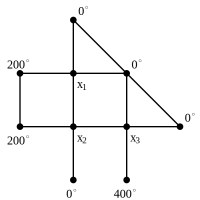
\includegraphics{Grid.eps}}
\caption{A grid of wires.}
\label{F:Grid}
\end{center}
\end{figure}
	\ba
	\item Determine equations for the temperatures $x_2$ and $x_3$ if the grid is in thermal equilibrium to construct a system of three linear equations in $x_1$, $x_2$, and $x_3$ that models node temperatures in the grid in thermal equilibrium.

	\item Use the method of elimination to find a specific solution to the system that makes sense in context.  

	\ea

\item We have seen that a linear system of two equations in two unknowns can have no solutions, one solution, or infinitely many solutions. Find, if possible, a specific example of each of the following. If not possible, explain why.
	\ba
	\item A linear system of three equations in two unknowns with no solutions.
	\item A linear system of three equations in two unknowns with exactly one solution.
	\item A linear system of three equations in two unknowns with exactly two solutions.
	\item A linear system of three equations in two unknowns with infinitely many solutions.
	\ea

\item We have seen that a linear system of three equations in three unknowns can have no solutions, one solution, or infinitely many solutions. Find, if possible, a specific example of each of the following. If not possible, explain why.
	\ba
	\item A linear system of two equations in three unknowns with no solutions.
	\item A linear system of two equations in three unknowns with exactly one solution.
	\item A linear system of two equations in three unknowns with exactly two solutions.
	\item A linear system of two equations in three unknowns with infinitely many solutions.
	\ea
		
\item Find a system of three linear equations in two variables $u$, $v$ whose solution is $u=2$, $v=1$.

\item Consider the system of linear equations
\begin{alignat*}{3}
x_1 	& {}+{} & hx_2 & {}={} & 2 \\
3x_1 	& {}+{} & 5x_2 & {}={} & 1 
\end{alignat*}
where $h$ is an unknown constant. 
	\ba
	\item  Determine the solution(s) of this system for all possible $h$ values, if a solution exists. (Note: Your answers for the variables will depend on the $h$.)
	\item How do your answers change if the second equation in the system above is changed to $3x_1+5x_2=6$?\\
	
	\ea
	
\item Suppose we are given a system of two linear equations
\begin{alignat}{4}
x_1 	& {}+{} & 2x_2 	& {}-{} 	& x_3{}={} 	& { } &1&{} \label{eq_1} \\
3x_1 	& {}+{} & x_2 	& {}+{} 	& 2x_3{}={} 	& {-} &1&. \label{eq_2} 
\end{alignat}
Find another system of two linear equations $E_1$ and $E_2$ in the variables $x_1$, $x_2$, and $x_3$ that are not multiples of each other or of equations (\ref{eq_1}) or (\ref{eq_2}) so that any solution $(x_1, x_2, x_3)$ to the system (\ref{eq_1}) and (\ref{eq_2}) is a solution to the system $E_1$ and $E_2$. 

\ee

\csection{True/False Questions}

In many sections you will be given True/False questions. In each of the True/False questions, you will be given a statement, such as ``if we add corresponding sides of two linear equations, then the resulting equation is a linear equation" and ``one can find a system of two equations in two unknowns that has infinitely many solutions." Your task will be to determine the truth value of the statement and to give a brief justification for your choice.



Note that a {\em general} statement is considered {\em true} only when it is always true. For example, the first of the above statements -- ``if we add corresponding sides of two linear equations, then the resulting equation is a linear equation" -- is a general statement. For this statement to be true, the equation we obtain by adding corresponding sides of any two linear equations has to be linear. If we can find two equations that do not give a linear equation when combined in this way, then this statement is false.



Note that an {\em existential} statement is considered {\em true} if there is at least one example which makes is true. For example, the latter of the above statements -- ``one can find a system of two equations in two unknowns that has infinitely many solutions" -- is an existential statement. For this statement to be true, existence of a system of two equations in two unknowns with infinitely many solutions should suffice. If it is impossible to find two such equations, then this statement is false.



To justify that something always happens or never happens, one would need to refer to other statements whose truth is known, such as theorems, definitions. In particular, giving an \textbf{example} of two linear equations that produce a linear equation when we add corresponding sides \emph{does not justify} why the sum of \textbf{any} two linear equations is also linear. Using the definition of linear equations, however, we can justify why this new equation will always be linear: each side of a linear equation is linear, and adding linear expressions always produces a linear sum. 



To justify that there are examples of something happening or not happening, one would need to give a specific example. For example, in justifying the claim that there is a system of two equations in two unknowns with infinitely many solutions, it is not enough to say ``An equation in two unknowns is a line in the $xy$-plane, so there can be two equations with the same line as their solution." In general, you should avoid the words ``can," ``possibly," ``maybe," etc., in your justifications. Instead, giving an example such as ``The linear system $x+y=1$ and $2x+2y=2$ of two equations in two unknowns has infinitely many solutions since the second equation gives the same line as the first in the $xy$-plane." provides complete justification beyond a reasonable doubt.


Each response to a True/False statement should be more than just True or False. It is important that you provide \textbf{justification} for your responses. 

\be
\item 
	\ba
	\item \textbf{True/False} The set of all solutions of a linear equation can be represented graphically as a line.


	\item \textbf{True/False} The set of all solutions of a linear equation in two variables can be represented graphically as a line.


	\item \textbf{True/False} The set of all solutions of an equation in two variables can be represented graphically as a line.


	\item \textbf{True/False} A system of three linear equations in two unknowns cannot have a unique solution. 


	\item \textbf{True/False} A system of three linear equations in three unknowns has a unique solution.

	\ea
\ee

\csection{Project: Modeling an Electrical Circuit and the Wheatstone Bridge Circuit} \label{sec:1_a_circuits}

Mathematical modeling, or the act of creating equations to model given information, is an important part of problem solving. In this section we will see how we derived the system of equations  
\begin{alignat}{4}
{}I_1 \	&- \	&{}I_2 \	&+ \	&{}I_3 \	&= 0  \notag \\ %\label{eq:circuit_1} \\
5I_1 \	&+ \	&2I_2 \		&{} \ 	&{}  \		&= 8 \notag \\ %\label{eq:circuit_2} \\
	\	&{} \ 	&2I_2 \		&+ \	&4I_3 \		&= 5 \notag %\label{eq:circuit_3}
\end{alignat}
to represent the electrical current in the circuit shown in Figure \ref{F:circuit1}. Recall that a circuit consists of  
\begin{itemize}
\item one or more electrical sources (like a battery), denoted by \ \ \  \resizebox{!}{0.25in}{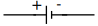
\includegraphics{1_a_pa_source}}
\item one or more resistors (like any appliance that you plug into a wall outlet), denoted by\\
\resizebox{!}{0.25in}{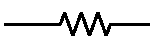
\includegraphics{1_a_pa_resistor}}.
\end{itemize}

The source creates a charge that produces potential energy $E$ measured in volts (V). No substance conducts electricity perfectly, there is always some price to pay (energy loss) to moving electricity. Electrical current $I$ in amperes (A) is the flow of the electric charge in the circuit. (A current of 1 ampere means that $6.2 \times 10^{18}$ electrons pass through the circuit per second.) Current flows out of the positive terminal of a source and runs through each branch of the circuit. Let $I_1$ be the current flowing through the upper branch, $I_2$ the current through middle branch, and $I_3$ the current through the lower branch as illustrated in Figure \ref{F:circuit1}. The goal is to find the current flowing in each branch of the circuit.  

Linear algebra comes into play when analyzing a circuit based on the relationship between current, resistance, and potential. Three basic principles govern current low in a circuit.
\begin{enumerate}
\item Resistance $R$ in ohms ($\Omega$) can be thought of as a measure of how difficult it is to move a charge along a circuit. When a current flows through a resistor, it must expend some energy, called a \emph{voltage drop}. Ohm's Law\index{Ohm's Law} states that the voltage drop $E$ across a resistor is the product of the current $I$ passing through the resistor and the resistance $R$. That is,
\[E = IR.\]
\item Kirchoff's Current Law\index{Kirchoff's Current Law} states that at any point in an electrical circuit, the sum of currents flowing into that point is equal to the sum of currents flowing out of that point.
\item Kirchoff's Voltage Law\index{Kirchoff's Voltage Law} says that around any closed loop the sum of the voltage drops is equal to the sum of the voltage rises. 
\end{enumerate} 

To see how these laws allow us to model the circuit in Figure \ref{F:circuit1}, we will need three equations in $I_1$, $I_2$, and $I_3$ to determine the values of these currents. Let us first apply Kirchoff's Current Law to the point P. The currents flowing into point P are $I_1$ and $I_3$, and the current flowing out is $I_2$. This produces the equation $I_1+I_3 = I_2$, or 
\[I_1 - I_2 + I_3 = 0.\]

\begin{pactivity} Apply Kirchoff's Current Law to the point $Q$ to obtain an equation in $I_1$, $I_2$, and $I_3$. What do you notice?
\end{pactivity}

We have three variables to determine, so we still need two more equations in $I_1$, $I_2$, and $I_3$. Next we apply Kirchoff's Voltage Law to the top loop in the circuit in Figure \ref{F:circuit1}. We will assume the following sign conventions:
\begin{itemize}
\item A current passing through a resistor produces a voltage drop if it flows in the direction of loop (and a voltage rise if the current passes in the opposite direction of the loop). 
\item A current passing through a source in the direction of the loop produces a voltage drop if it flows from $+$ to $-$ and a voltage rise if it flows from $-$ to $+$, while a current passing through a source in the opposite direction of the loop produces a voltage rise if it flows from $+$ to $-$ and a voltage drop if it flows from $-$ to $+$. 
\end{itemize}
(The directions chosen in Figure \ref{F:circuit1} for the voltage flow are arbitrary -- if we reverse the flow then we just replace voltage drops with voltage rises and obtain the same equations. If a solution shows that a current is negative, then that current flows in the direction opposite of what is shown.) 

If we move in the counterclockwise direction around the top loop in the circuit in Figure \ref{F:circuit1}, there is a voltage rise through the source of 8 volts. This must equal the voltage drop in this loop. The current $I_1$ passing though the resistor of resistance 2 $\Omega$ produces a voltage drop of $2I_1$ volts. Similarly, the current $I_1$ passing through the resistor of resistance $3 \Omega$ produces a voltage drop of $3I_1$ volts. Finally, the current $I_2$ passing through the resistor of resistance 2 $\Omega$ produces a voltage drop of $2I_2$ volts. So Kirchoff's Voltage Law applied to the top loop in the circuit in Figure \ref{F:circuit1} gives us the equation $2I_1 + 3I_1 + 2I_2 = 8$ or 
\[5I_1 + 2I_2 = 8.\]

\begin{pactivity} Apply Kirchoff's Voltage Law to the bottom loop in the circuit in Figure \ref{F:circuit1} to obtain an equation in $I_1$, $I_2$, and $I_3$. Compare the three equations we have found to those in the introduction.
\end{pactivity}
 
\begin{figure}[h]
\begin{center}
\resizebox{!}{2.0in}{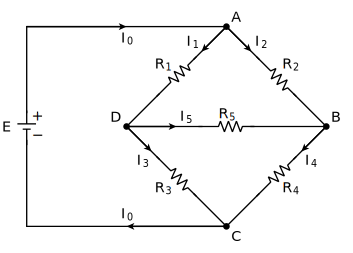
\includegraphics{Wheatstone}}
\end{center}
\caption{A Wheatstone bridge circuit.}
\label{F:Wheatstone}
\end{figure}

\begin{pactivity} Consider the circuit as shown in Figure \ref{F:Wheatstone}, with a single source and five resistors with resistances $R_1$, $R_2$,  $R_3$, $R_4$, and $R_5$ as labeled. 
\ba
\item Assume the following information. The voltage $E$ is $13$ volts, $R_1=R_2=R_3=R_5= 1 \Omega$, and $R_4 = 2  \Omega$. Follow the directions given to find the currents $I_0$, $I_1$, $I_2$, $I_3$, $I_4$, and $I_5$. 
	\begin{enumerate}[i.]
	\item Use Kirchoff's Current Law to show that $I_0 = I_1+I_2$, $I_3 = I_1-I_5$, and  $I_4 = I_2 + I_5$. Thus, we reduce the problem to three variables. 

	\item Apply Kirchoff's Voltage Law to three loops to show that the currents must satisfy the linear system 
\begin{alignat}{4}
{2}I_1	&{}{}		&{}	 	&{}-{}	&{}I_5 	&= & \ 13&{}   \label{eq:Wheatstone_1} \\ 
{}	 	&{}{}		&{3}I_2 	&{}+{}	&{2}I_5 	&= & \ 13&{}  \label{eq:Wheatstone_2}  \\ 
{}I_1 	&{}-{}	&{}I_2 	&{}+{}	&{}I_5 	&= & \ 0&{.}   \label{eq:Wheatstone_3} 
\end{alignat}

	\item Solve the system to find the unknown currents.
	

	\end{enumerate}

\item The circuit pictured in Figure \ref{F:Wheatstone} is called a \emph{Wheatstone bridge} (invented by Samuel Hunter Christie in 1833 and popularized by Sir Charles Wheatstone in 1843). The Wheatstone bridge is a circuit designed to determine an unknown resistance by balancing two paths in a circuit. It is set up so that the resistances of resistors $R_1$ and $R_2$ are known, $R_3$ is a variable resistor and we want to find the resistance of $R_4$. The resistor $R_5$ is replaced with a voltmeter, and the resistance of $R_3$ is varied until the voltmeter reads $0$. This balances the circuit and tells the resistance of resistor $R_4$. Show that if the current $I_5$ in Figure \ref{F:Wheatstone} is $0$ (so the circuit is balanced), then $R_4 = \frac{R_2R_3}{R_1}$ (which is how we calculate the unknown resistance $R_4$). Do this in general and do not use any specific values for the resistances or the voltage. 


\ea
\end{pactivity}


